\chapter{EIGRP}

\section{Basic features}

Features of EIGRP:

\begin{itemize}
\item Use DUAL algorithm
\item Use RTP  instead of TCP or UDP
\item Partial and Bounded Updates -- Sends updates only when there is a change and only to the routers that need the information
\item Supports Equal and Unequal cost load balancing
\item Does not encrypt the routing updates
\item \textbf{Authentication:} Only accepts routing information from other routers with the same authentication information 
\end{itemize}

\paragraph{Protocol Dependent Modules (PDM)}sends and receives EIGRP packets that are encapsulated in IPv4 or IPv6.

\paragraph{Reliable Transport Protocol (RTP)}EIGRP was designed as a network layer independent routing protocol. Because of this design, EIGRP cannot use UDP or TCP, but use RTP instead. RTP includes both reliable and unreliable delivery of EIGRP packets, similar to TCP and UDP, respectively. RTP can send EIGRP packets as unicast or multicast. EIGRP multicast address is 224.0.0.10 for IPv4 and  FF02::A for IPv6.

\section{Packet types}

\subsection{Hello packets}

EIGRP uses small Hello packets to discover other EIGRP-enabled routers on directly connected links. Hello packets are used by routers to form EIGRP neighbor adjacencies.\\
 
Hello packets are sent as multicast packets \emph{every five seconds}. However, on slow network (e.g. multipoint, NBMA networks with access links of T1), Hello packets are sent as unicast packets every 60 seconds.\\
 
EIGRP uses a Hold timer to determine the maximum time the router should wait to receive the next Hello before declaring that neighbor as unreachable. By default, the hold time is \emph{three times the Hello interval}. If the hold time expires, EIGRP declares the route as down and DUAL searches for a new path by sending out queries.

\subsection{Update packets}
EIGRP sends Update packets to propagate routing information. Update packets are sent only when necessary. EIGRP updates contain only the routing information needed and are sent only to those routers that require it.\\
 
EIGRP uses \emph{partial update} and \emph{bounded update}. A partial update means that the update only includes information about route changes. A bounded update refers to the sending of partial updates only to the routers that are affected by the changes. Bounded updates help EIGRP minimize the bandwidth that is required to send EIGRP updates.

\subsection{Acknowledgment packets}
EIGRP sends Acknowledgment (ACK) packets when reliable delivery is used. An EIGRP acknowledgment is an EIGRP Hello packet without any data. RTP uses reliable delivery for Update, Query, and Reply packets.
\subsection{Query and reply packets}
DUAL uses Query and Reply packets when searching for networks and other tasks. Queries and replies use reliable delivery. Queries can use multicast or unicast, whereas replies are always sent as unicast.
\section{Encapsulating EIGRP Messages}
\subsection{TLV fields}
The data portion of an EIGRP message is encapsulated in a packet (figure \ref{EIGRP-packet-header}). This data field is called \emph{type}, \emph{length}, \emph{value} (TLV). The \emph{type}s of TLVs relevant to this course are EIGRP parameters (figure \ref{EIGRP-parameters}), IP internal routes (figure \ref{EIGRP-internal-route}), and IP external routes (figure \ref{EIGRP-external-route}). The \emph{length} field identifies the size (in bytes) of the \emph{value} field. The \emph{value} field contains data for EIGRP message.\par 
The EIGRP parameters include the weights that EIGRP uses for its composite metric (K1 -- K5). By default, only bandwidth and delay are weighted. Both are weighted equally; therefore, the K1 field for bandwidth and the K3 field for delay are both set to one (1). The other K values are set to zero (0).\par 
Each IP internal routes and IP external routes contains one route entry and the metric information for that route. The Update packet parameters identify IP internal and external routes. The IP internal message is used to advertise EIGRP routes within an autonomous system, whereas the IP external message is used to import default static route, as well as routes outside the autonomous system, into the EIGRP routing process.
\subsection{Packet header}
In the packet header (figure \ref{EIGRP-packet-header}), the protocol field is set to 88 to indicate EIGRP, and the destination address is set to the multicast 224.0.0.10 for IPv4, and FF02::A for IPv6. If the EIGRP packet is encapsulated in an Ethernet frame, the destination MAC address is also a multicast address, 01-00-5E-00-00-0A.\par 
Another important field in the packet header is opcode field, which specifies EIGRP packet type. Specifically, it identifies the EIGRP messages as either type 1 = Update, type 3 = Query, type 4 = Reply, type 5 = Hello. \par 
The autonomous system number specifies the EIGRP routing process. Unlike RIP, multiple instances of EIGRP can run on a network. The autonomous system number is used to track each running EIGRP process.\par 
\begin{figure}[hbtp]
\centering
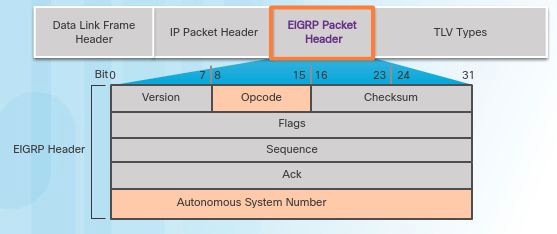
\includegraphics[width=0.6\textwidth]{pictures/EIGRP-packet-header.png}
\caption{EIGRP packet header} \label{EIGRP-packet-header}
\end{figure}
\begin{figure}[hbtp]
\centering
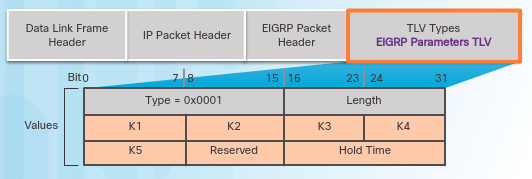
\includegraphics[width=0.6\textwidth]{pictures/EIGRP-parameters.png}
\caption{EIGRP paramters TLV fields} \label{EIGRP-parameters}
\end{figure}
\begin{figure}[hbtp]
\centering
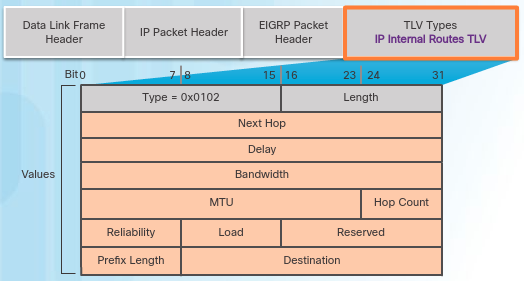
\includegraphics[width=0.6\textwidth]{pictures/EIGRP-internal-route.png}
\caption{EIGRP internal routes TLV fields} \label{EIGRP-internal-route}
\end{figure}
\begin{figure}[hbtp]
\centering
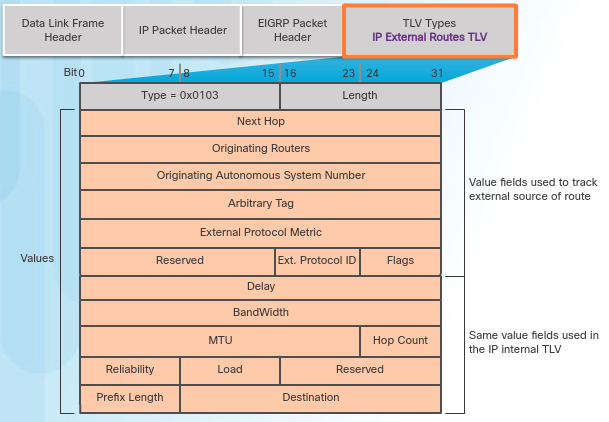
\includegraphics[width=0.6\textwidth]{pictures/EIGRP-external-route.png}
\caption{EIGRP external route TLV fields} \label{EIGRP-external-route}
\end{figure}
\section{Operation}
\subsection{Neighbor adjacency}
EIGRP uses Hello packets to establish and maintain neighbor adjacencies. To accomplish this, two EIGRP routers must use the same EIGRP metric parameters (K values) and both must be configured using the same autonomous system number.\par 
Each EIGRP router maintains a neighbor table, which contains a list of routers on shared links that have an EIGRP adjacency with this router. The neighbor table is used to track the status of these EIGRP neighbors.\par 
When a new router A comes up on the link and it floods hello packets through all of its EIGRP-configured interfaces. The neighbor routers receive those packets, adds A to their neighbor tables, and sends hello as well as update packets to A. Router A, then add those routers to its neighbor table and updates its topology table with information from received packets.
\subsection{Topology table}
Each EIGRP router maintains a topology table for each routed protocol configured, such as IPv4 and IPv6. The topology table includes route entries for every destination that the router learns from its directly connected EIGRP neighbors.\par 
When a router receives the EIGRP update from neighbor, it adds all update entries to its topology table. Because EIGRP update packets use reliable delivery, the router replies with an EIGRP acknowledgment packet informing its neighbors that it has received the update.
\subsection{Metric}
By default, EIGRP uses the following values in its composite metric to calculate the preferred path to a network:
\begin{itemize}
\item \textbf{Bandwidth} -- The slowest bandwidth among all of the outgoing interfaces, along the path from source to destination.
\item \textbf{Delay} -- The cumulative (sum) of all interface delay along the path (in tens of microseconds).
\end{itemize}
Default composite formula:
\[ \text{metric} = \left( K1\times\text{bandwidth} + K1\times\text{bandwidth} \right) \times 256 \]
Complete composite formula:
\[ \text{metric} = \left( K1\times\text{bandwidth} + \frac{K2\times\text{bandwidth}}{256\times\text{load}} + K3\times\text{delay} \right) \times \frac{K5}{K4+\text{reliability}} \times 256 \]
This is a conditional formula. If $K5=0$, the last term is replaced by 1. Default values for each parameter:
\begin{itemize}
\item K1 (bandwidth) = 1
\item K2 (load) = 0
\item K3 (delay) = 0
\item K4 (reliability) = 0
\item K5 (reliability) = 0
\end{itemize}
\subsubsection{Bandwidth}
EIGRP uses the slowest bandwidth along the path to the destination network. EIGRP divides a reference bandwidth value of $10^7$ by the interface bandwidth value in kb/s. If the result is not a whole number, then the value is rounded down. For example, $10^7$ divided by 1024 equals 9765.625. The .625 is dropped to yield 9765 for the bandwidth portion of the composite metric.
\subsection{Delay}
EIGRP uses the sum of all delays along the path to the destination. The sum of these delays is divided by 10. See also table \ref{delay-value} for default delay values \par 
For example, along the path R1$\rightarrow$R2$\rightarrow$R3, the Serial 0/0/1 interface on R2 has a delay of 20,000 microseconds, the Gigabit 0/0 interface on R3 has a delay of 10 microseconds. The delay is $ \left( 20000 + 10 \right) \div 10 = 2001 $.
\begin{table}[h!]
\centering
\caption{Default delay values}
\label{delay-value}
\begin{tabular}{|l|l|}
\hline
Media            & Delay \\ \hline
Ehternet         & 1000  \\ \hline
Fast Ethernet    & 100   \\ \hline
Gigabit Ethernet & 10    \\ \hline
Serial link      & 20000 \\ \hline
\end{tabular}
\end{table}
\subsection{DUAL algorithm}
EIGRP uses the Diffusing Update Algorithm (DUAL) to provide the best loop-free path and loop-free backup paths. DUAL uses several terms, which are discussed in more detail throughout this section:
\begin{itemize}
\item Successor -- A successor is a neighboring router that is used for packet forwarding and is the least-cost route to the destination network. The IP address of a successor is shown in a routing table entry right after the word via (see figure \ref{EIGRP-FD}). 
\item Feasible Distance (FD) -- FD is the lowest calculated metric to reach the destination network. FD is the metric listed in the routing table entry as the second number inside the brackets (see figure \ref{EIGRP-FD}). As with other routing protocols, this is also known as the metric for the route.
\item Feasible Successor (FS) -- An FS is a neighbor that has a loop-free backup path to the same network as the successor, and it satisfies the Feasibility Condition (FC). FS is not represented in the routing table until the Successor is down.
\item Reported Distance (RD) -- The RD is simply an EIGRP neighbor’s FD to the same destination network.
\item Feasible Condition or Feasibility Condition (FC) -- The FC is met when a neighbor’s RD to a network is less than the local router’s feasible distance to the same destination network. If the RD is less, it represents a loop-free path. 
\end{itemize}
\begin{figure}[hbtp]
\centering
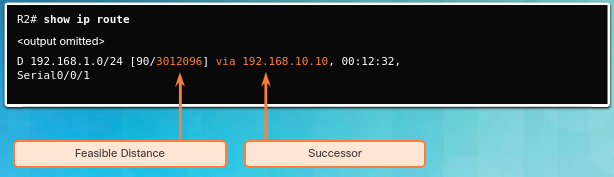
\includegraphics[scale=1]{pictures/EIGRP-FD.png}
\caption{Successor and Feasible Distance} \label{EIGRP-FD}
\end{figure}
The decision process for all route computations is done by the DUAL Finite State Machine (FSM). The DUAL FSM tracks all routes and uses EIGRP metrics to select efficient, loop-free paths, and to identify the routes with the least-cost path to be inserted into the routing table.\par 
Recomputation of the DUAL algorithm can be processor-intensive. EIGRP avoids recomputation whenever possible by maintaining a list of backup routes that DUAL has already determined to be loop-free. If the primary route in the routing table fails, the best backup route is immediately added to the routing table. \par
\begin{figure}[hbtp]
\centering
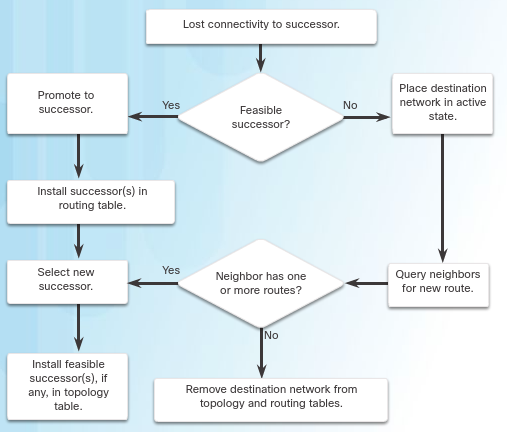
\includegraphics[width=0.7\textwidth]{pictures/EIGRP-DUAL.png}
\caption{DUAL Finite State machine} \label{EIGRP-DUAL}
\end{figure}
When the successor is no longer available and there is no feasible successor, DUAL puts the route into an active state. DUAL sends EIGRP queries asking other routers for a path to the network. Other routers return EIGRP replies, letting the sender of the EIGRP query know whether or not they have a path to the requested network. If none of the EIGRP replies have a path to this network, the sender of the query does not have a route to this network. See also figure \ref{EIGRP-DUAL}.
\section{Tune EIGRP}
\subsection{Automatic summarization}
Route summarization allows a router to group networks together and advertises them as one large group using a single, summarized route. Summarization decreases the number of entries in routing updates and lowers the number of entries in local routing tables. It also reduces bandwidth utilization for routing updates and results in faster routing table lookups.\par 
However, in classes IP network, the only way that all routers can find the best routes for each individual subnet is for neighbors to send subnet information. In this situation, automatic summarization should be disabled. When automatic summarization is disabled, updates include subnet information.\par 
A problem associated with automatic route summarization is that a summary address also advertises networks that are not available on the advertising router. For example, R1 is advertising the summary address 172.16.0.0/16, but it is only connected to 172.16.1.0/24. Therefore, R1 may receive incoming packets to destinations that do not exist (for example, 172.16.2.0/24). It then forwards a request to a destination network that does not exist, creating a routing loop.\\
EIGRP uses the Null0 interface to avoid this problem. The Null0 interface is a virtual IOS interface that is a route to nowhere. If R1 receives a packet destined for a network that is advertised by the classful mask but does not exist, it sends discards the packets by sending them to Null0.\par 
\note  The Null0 summary route is removed when autosummarization is disabled using the no auto-summary router configuration mode command.
\subsection{Hello and hold timers}
 The hold time tells the router the maximum time that the router should wait to receive the next Hello before declaring that neighbor as unreachable.Hello intervals and hold times are configurable on a per-interface basis and do not have to match with other EIGRP routers to establish or maintain adjacencies.\par 
If the Hello interval is changed, ensure that the hold time value is not less than, the Hello interval. Otherwise, neighbor adjacency goes down after the hold time expires and before the next Hello interval. 